\label{sec:gbb-results}

Figure~\ref{fig:gbb-results} presents a summary of the results. Generally we observe that the Sherpa predictions are closer to data, especially for low \zpt and \mpt. However both generators seem to show an opposite trend in $\dphi$ compared to data. The data distribution is upward curving in contrast to downward curving or flat distributions in MC. For \drbb, both generators show very good agreement with data. This study suggests further investigations of this kind or others to fully explore the quantities where disagreements between data and MC are prominent and are largely unconstrained. The truth level distributions are available at HEPdata\footnote{http://hepdata.cedar.ac.uk/} for MC tunning or different interpretations. 

\begin{figure}[htpb!]
\begin{center}
  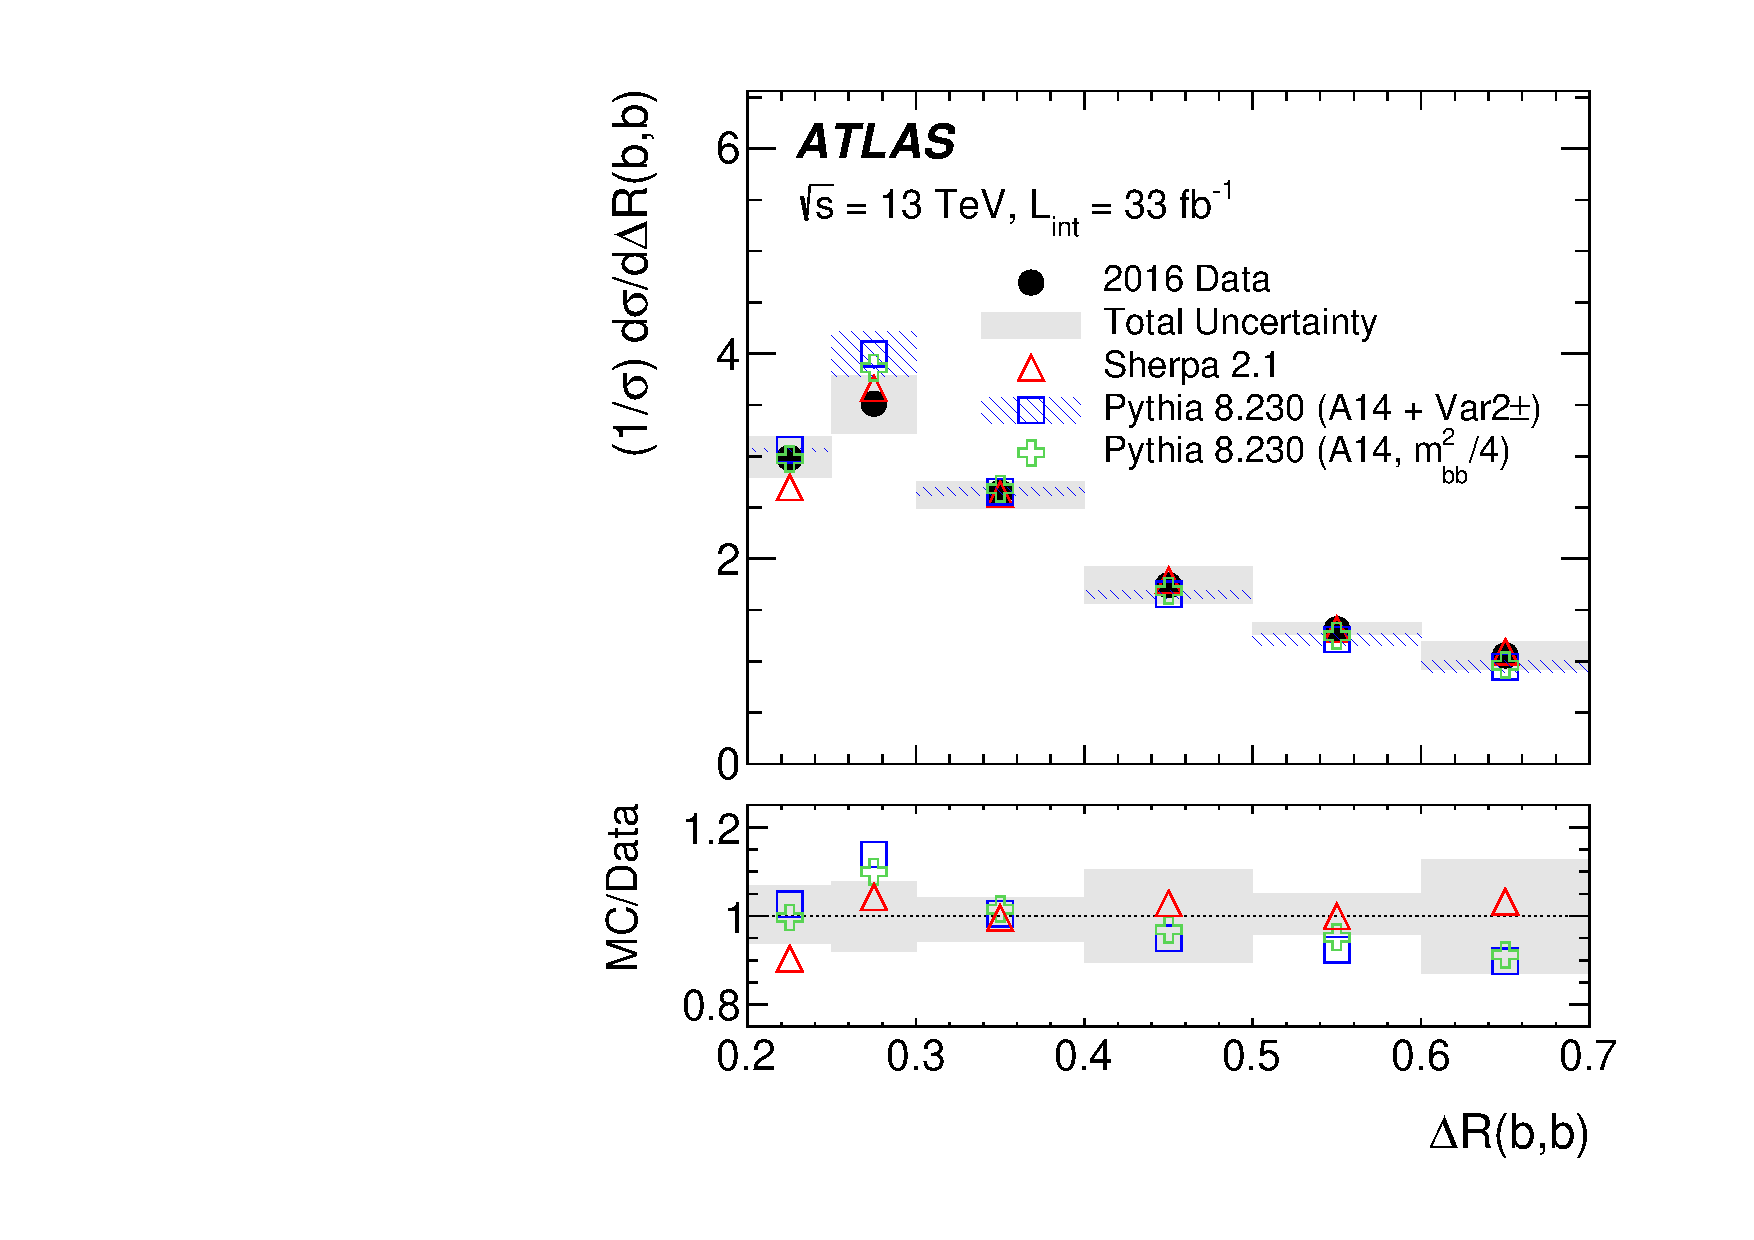
\includegraphics[width=0.45\linewidth]{figures/gbb/unfold_final_dR}
  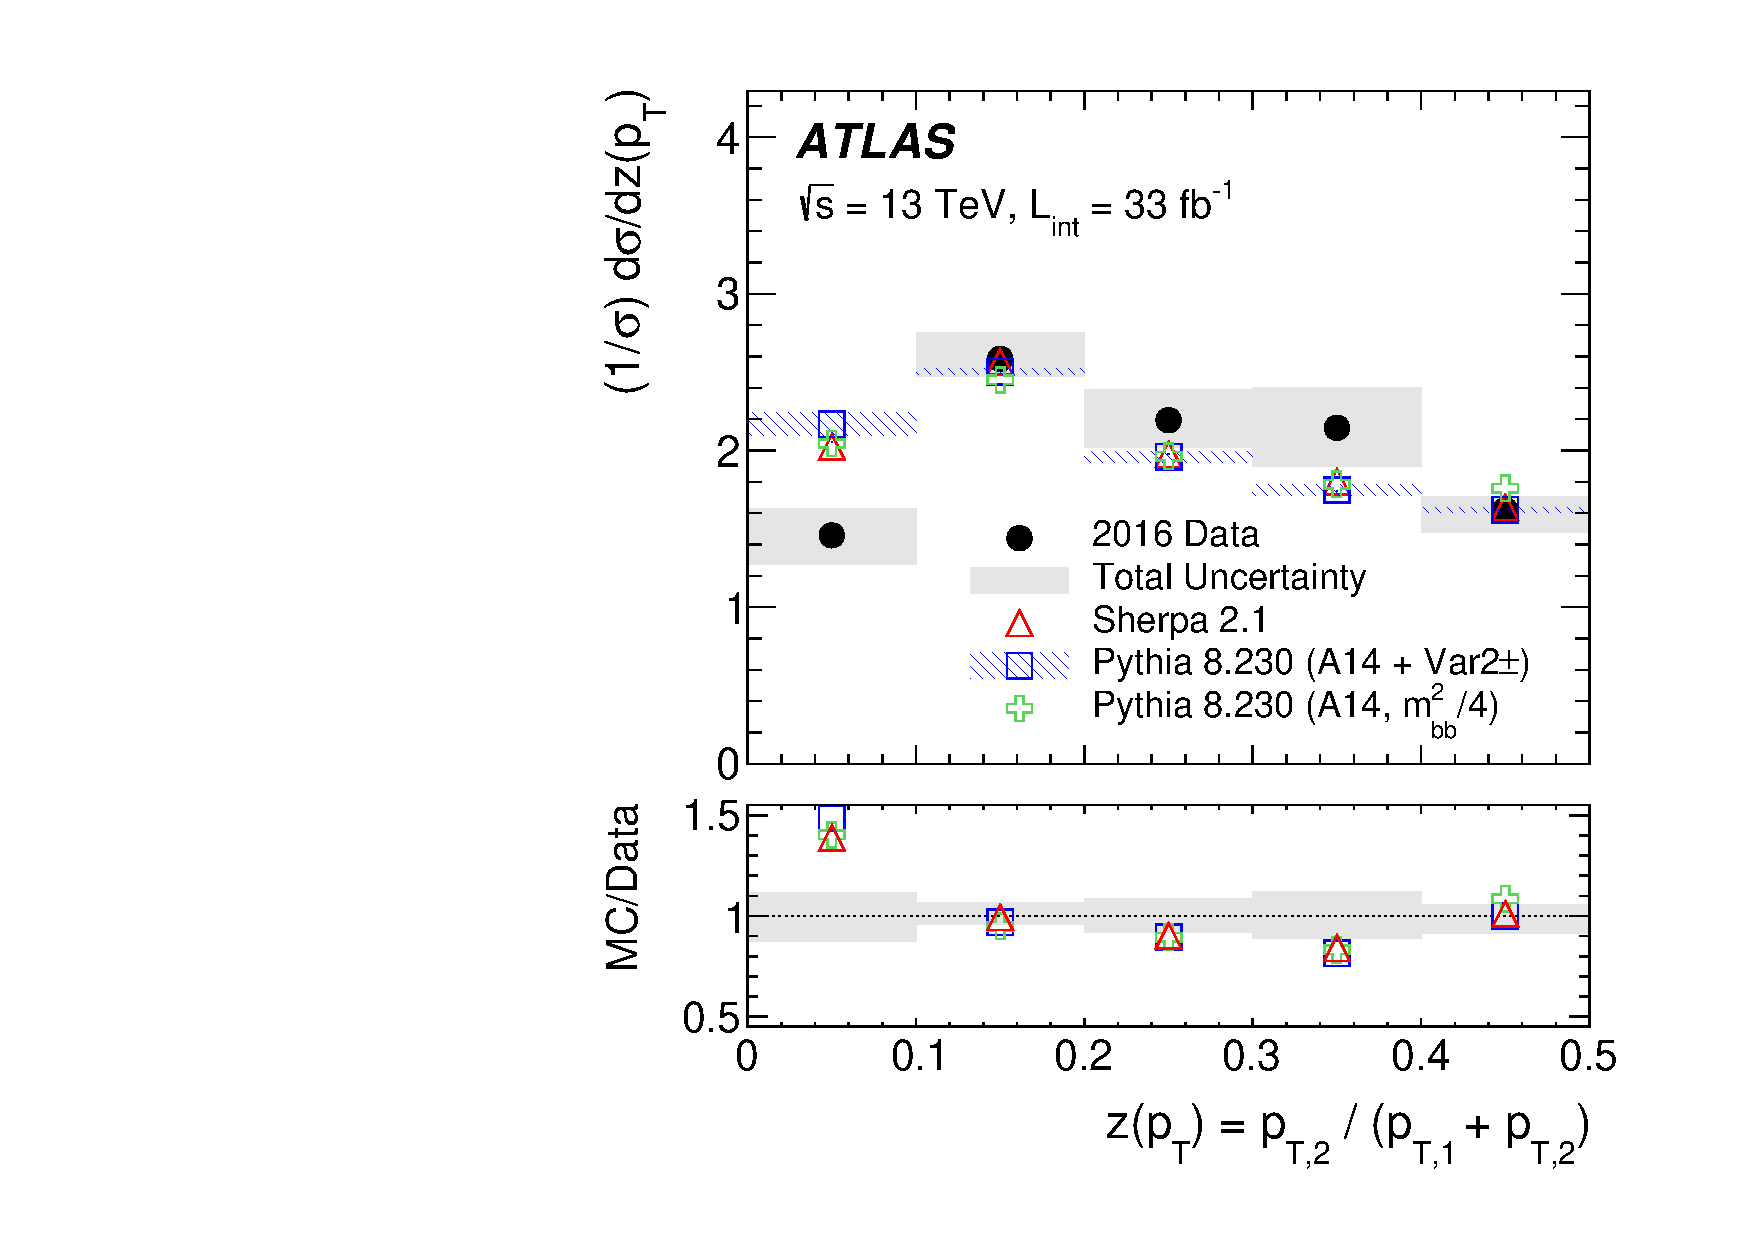
\includegraphics[width=0.45\linewidth]{figures/gbb/unfold_final_zpt}
  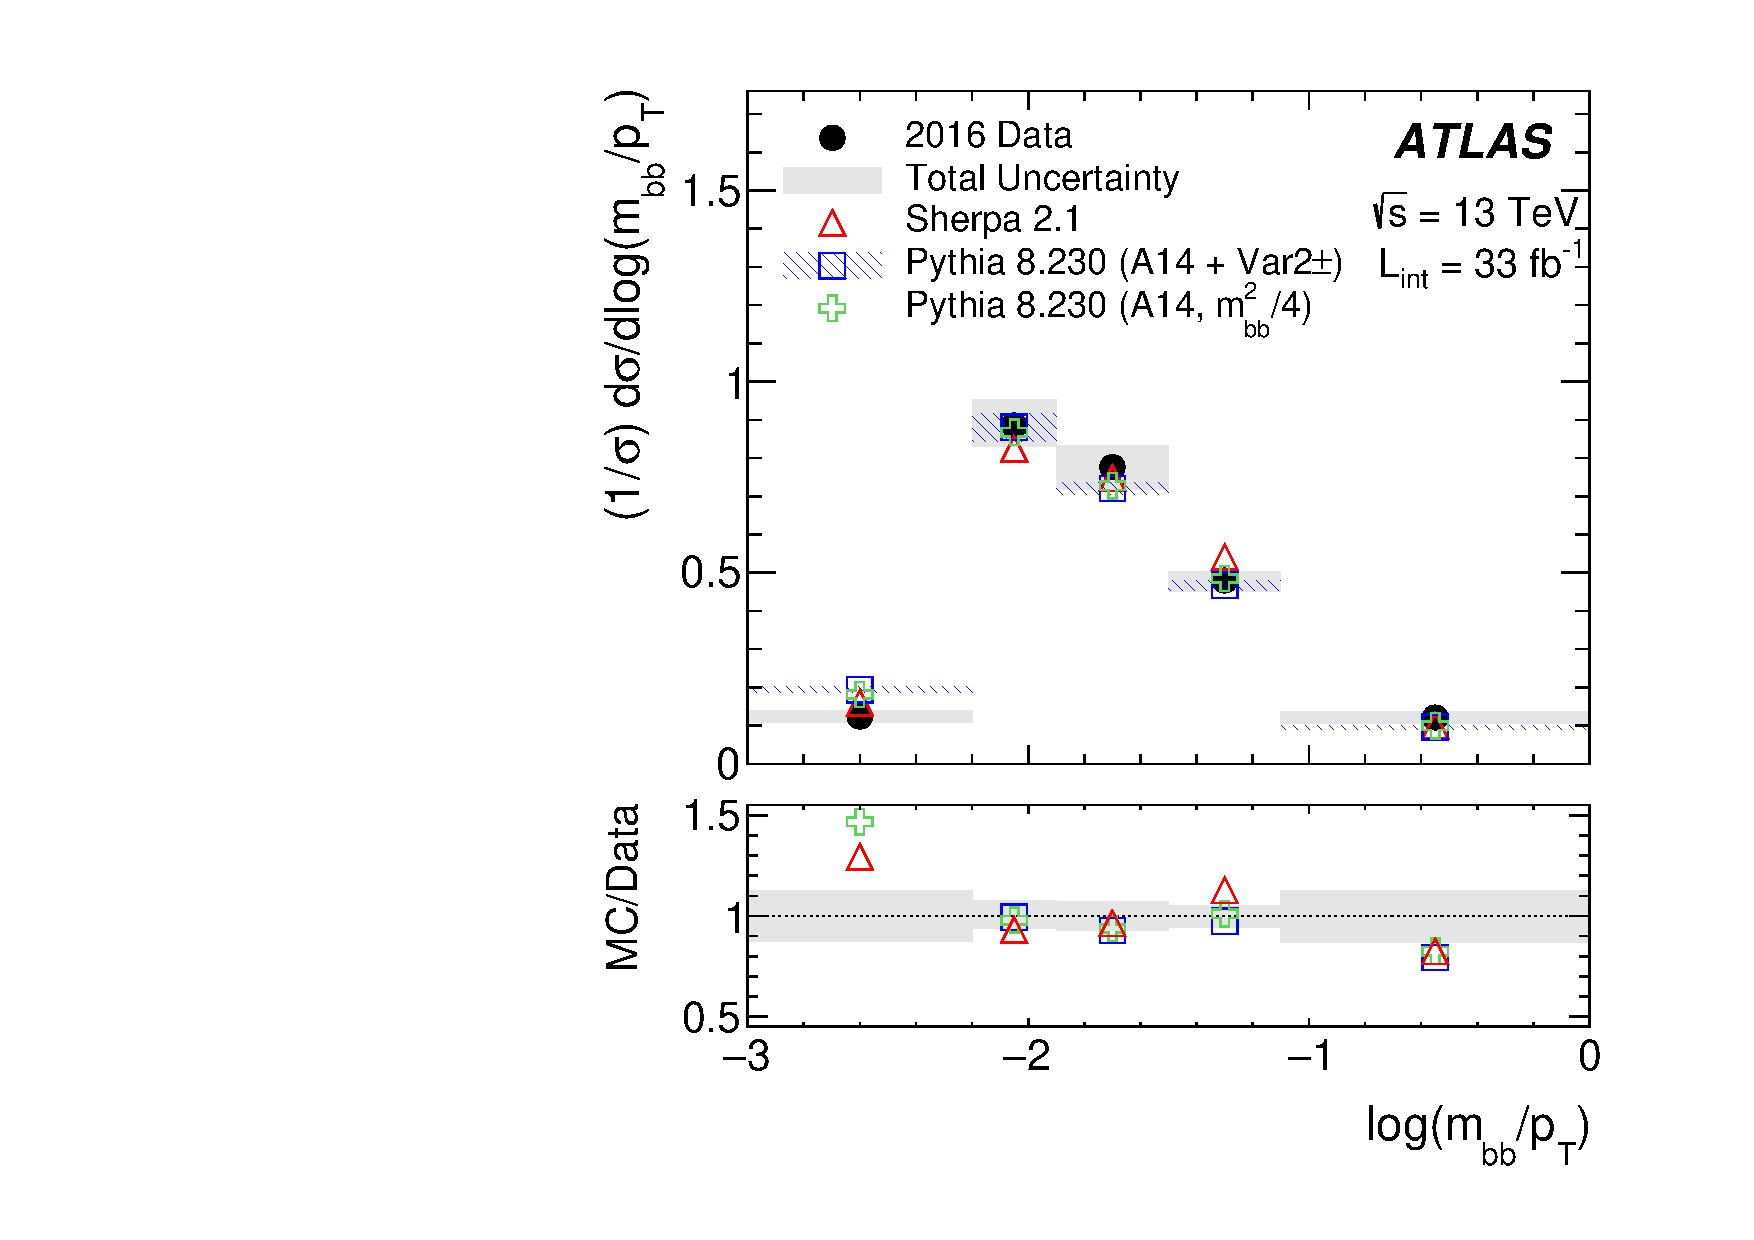
\includegraphics[width=0.45\linewidth]{figures/gbb/unfold_final_mass}
  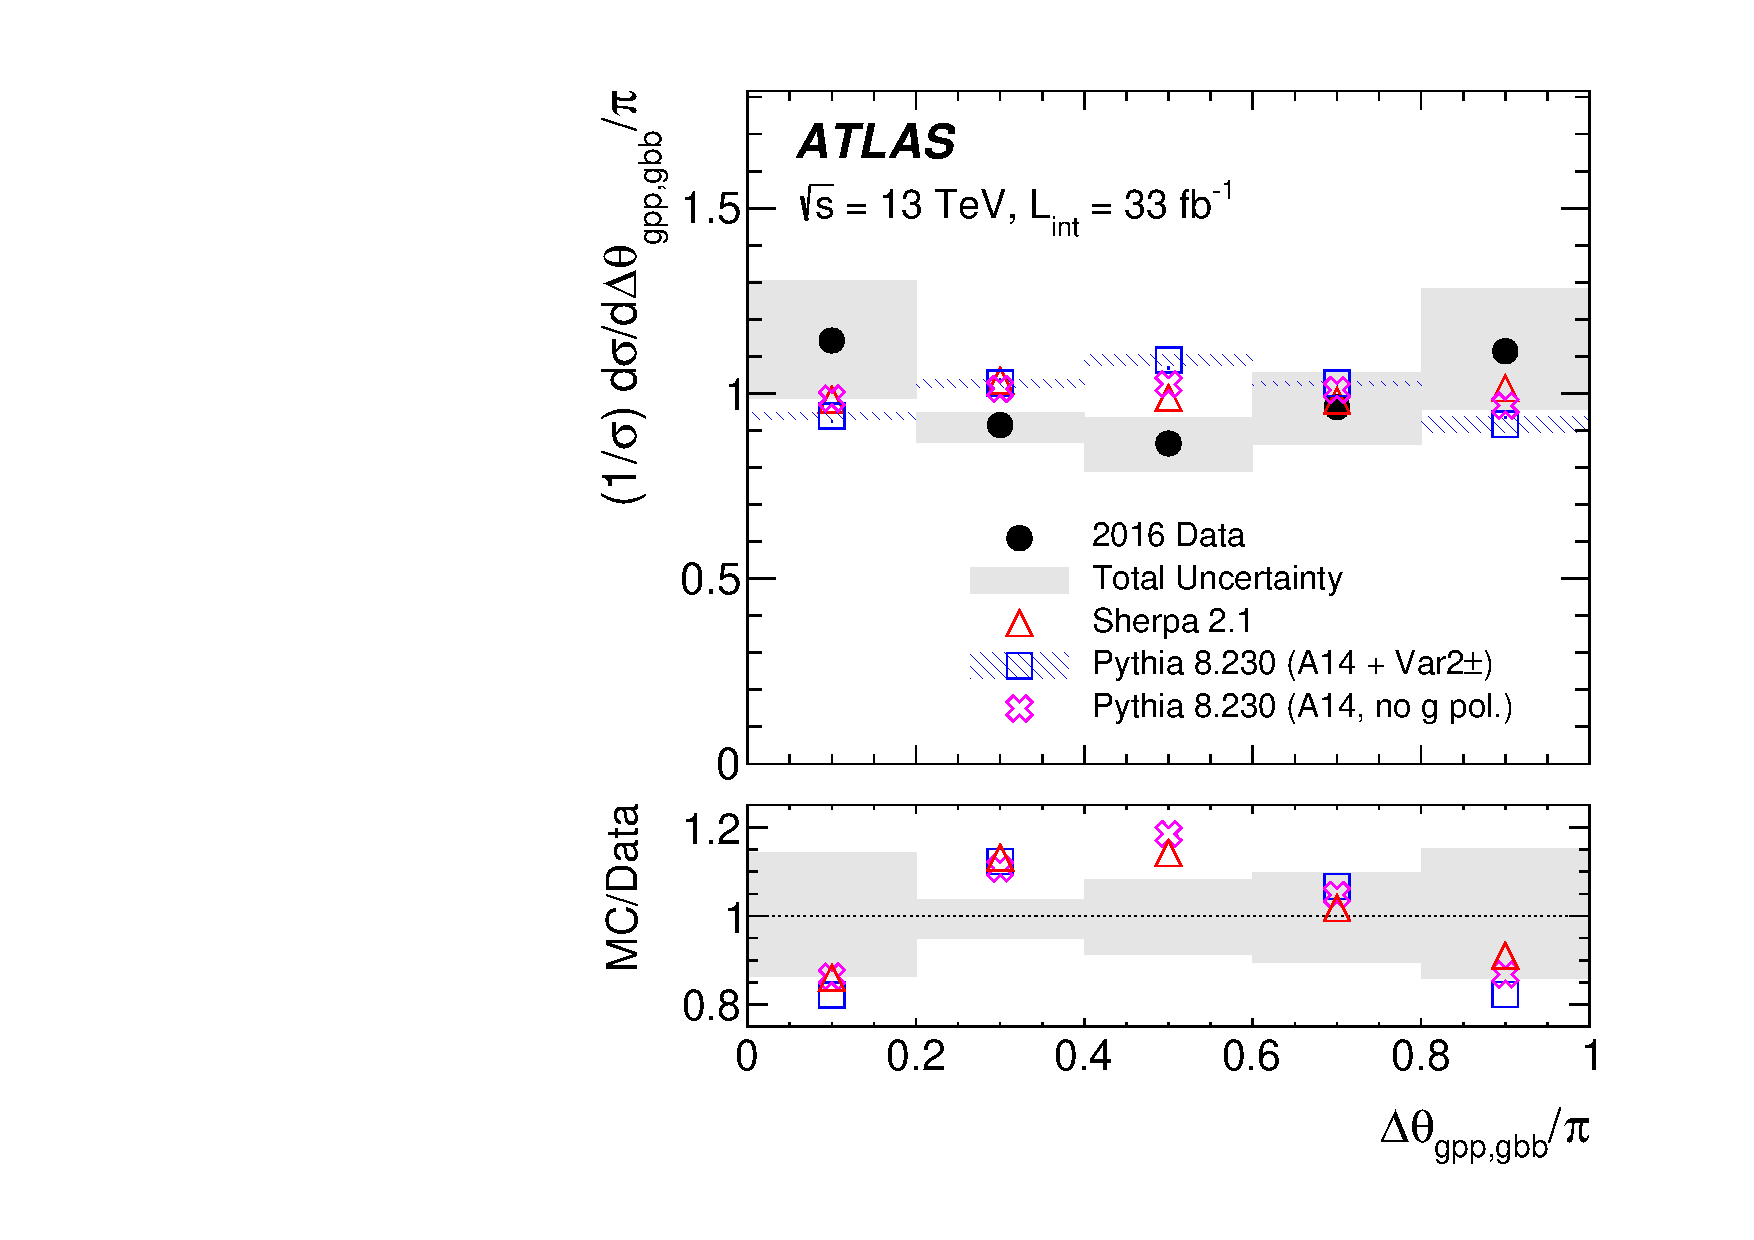
\includegraphics[width=0.45\linewidth]{figures/gbb/unfold_final_dtheta}
\caption[]{The unfolded data compared with Pythia. The data points have error bars that are the statistical uncertainties and the bands are the total systematic uncertainties. The bands for the Pythia prediction represented by a square indicate the variation of a $\pm10\%$ in the final state shower $\alpha_s$. The additional set of Pythia markers use $m_{b\bar b}^2/4$ for the renormalization scale or turns off gluon polarization.}
\label{fig:gbb-results}
\end{center}
\end{figure}


